\documentclass[conference]{IEEEtran}
\IEEEoverridecommandlockouts

\usepackage{cite}
\usepackage{amsmath,amssymb,amsfonts}
\usepackage{algorithmic}
\usepackage{graphicx}
\usepackage{textcomp}
\usepackage{xcolor}
\usepackage{booktabs}
\usepackage[utf8]{inputenc}
\usepackage[T1]{fontenc}
\usepackage{tikz}
\usetikzlibrary{shapes.geometric,arrows.meta,positioning,backgrounds,calc,fit}
\definecolor{amberbr}{RGB}{200,145,0}
\definecolor{bluebr} {RGB}{66,133,244}
\definecolor{tealbr} {RGB}{0,150,170}
\definecolor{greenbr}{RGB}{56,142,60}
\definecolor{redbr}  {RGB}{198,40,40}
\usepackage{array}
\usepackage{multirow}
\usepackage{placeins}

% Hifenização em português (evita quebras incorretas como "car-acterísticas").
% Os rótulos do IEEEtran são restaurados logo abaixo, pois o babel os traduziria.
\usepackage[brazilian]{babel}
\addto\captionsbrazilian{%
  \renewcommand{\figurename}{Fig.}%
  \renewcommand{\tablename}{TABLE}%
  \renewcommand{\refname}{References}%
  \renewcommand{\abstractname}{Abstract}%
}
\hyphenation{%
  ca-rac-te-rís-ti-cas con-vo-lu-cio-nais con-vo-lu-cio-nal
  to-mo-grá-fi-cas to-mo-gra-fia ar-qui-te-tu-ras ar-qui-te-tu-ra
  clas-si-fi-ca-ção clas-si-fi-ca-dor apren-di-za-do de-sem-pe-nho
  com-pu-ta-do-ri-za-da equa-li-za-ção me-to-do-lo-gia
  re-pro-du-ti-bi-li-da-de nor-ma-li-za-ção in-ten-si-da-des
}

\definecolor{darkblue}{HTML}{00005C}
\usepackage[colorlinks=true, citecolor=darkblue, linkcolor=darkblue, urlcolor=darkblue]{hyperref}

\def\BibTeX{{\rm B\kern-.05em{\sc i\kern-.025em b}\kern-.08em
    T\kern-.1667em\lower.7ex\hbox{E}\kern-.125emX}}

\begin{document}

\title{Análise Comparativa de Arquiteturas de CNNs com Técnicas de
Pré-processamento para Classificação de Câncer Renal em Imagens
Tomográficas}

\author{
\IEEEauthorblockN{Thiago Cordeiro de Melo}
\IEEEauthorblockA{
    \textit{Escola Superior de Tecnologia}\\
    \textit{Universidade do Estado do Amazonas}\\
    Manaus, Brasil\\
    thiago.melo@uea.edu.br
}
\and
\IEEEauthorblockN{Wheidima Carneiro de Melo}
\IEEEauthorblockA{
    \textit{Escola Superior de Tecnologia}\\
    \textit{Universidade do Estado do Amazonas}\\
    Manaus, Brasil\\
    wmelo@uea.edu.br
}
}

\maketitle

% ─────────────────────────────────────────────────────────────────────────────
\begin{abstract}
O câncer renal é uma das neoplasias urológicas de maior mortalidade, com
diagnóstico frequentemente tardio. Este trabalho investiga o impacto de duas
técnicas de pré-processamento de contraste --- CLAHE e correção gama
(com fator gama igual a 0,7) --- em comparação com a condição base sobre cinco
arquiteturas de Redes Neurais Convolucionais com aprendizado por
transferência: ResNet-18, ResNet-34, ResNet-50, AlexNet e VGG-16.
O conjunto de dados empregado é o CT Kidney Dataset, com 4.566 imagens
balanceadas entre as classes Normal e Tumor, divididas nas proporções
60/20/20 para treino, validação e teste. Os resultados demonstram que a
correção gama melhora ou mantém estável o desempenho em todas as arquiteturas
avaliadas, ao passo que o CLAHE apresenta comportamento inconsistente,
reduzindo a acurácia das redes mais rasas. O melhor resultado global foi
obtido pela VGG-16 com correção gama, que alcançou 99,12\% de acurácia
e revocação de 100\% para a classe Tumor.
\end{abstract}

\begin{IEEEkeywords}
Classificação de Câncer Renal, Redes Neurais Convolucionais, Equalização de
Histograma, CLAHE, Correção Gama, Aprendizado Profundo, Imagens Tomográficas
\end{IEEEkeywords}

% ─────────────────────────────────────────────────────────────────────────────
\section{Introdução}

O diagnóstico precoce configura-se como elemento determinante para o êxito
terapêutico em oncologia, repercutindo de forma direta sobre a sobrevida e
o bem-estar dos pacientes~\cite{gomes2025}. Dentre as neoplasias de maior
relevância clínica, o câncer renal destaca-se como a neoplasia urológica de
maior letalidade~\cite{santos2025}, manifestando-se predominantemente em
indivíduos na faixa etária de $50$ a $70$ anos. No Brasil, foram registrados
aproximadamente $13.000$ novos casos e mais de $4.000$ óbitos no ano de
$2020$~\cite{inca2022}. Não obstante, a inespecificidade sintomatológica nos
estágios iniciais, associada à reduzida eficácia das estratégias de
rastreamento populacional, compromete a identificação precoce da
enfermidade~\cite{campbell2021}. Em razão disso, parcela considerável dos
casos é diagnosticada em fases avançadas, o que restringe de maneira
substancial as possibilidades de intervenção terapêutica eficaz.

As consequências desse diagnóstico tardio tornam-se mais graves em virtude do
papel essencial exercido pelos rins no organismo, responsáveis por funções
como a filtração de metabólitos, a regulação da pressão arterial e a produção
de hormônios fundamentais, a exemplo da eritropoietina~\cite{hall}. À medida
que o câncer renal avança, essas funções podem ser severamente comprometidas,
tornando necessários tratamentos invasivos como hemodiálise e nefrectomia,
podendo a doença evoluir, nos casos mais graves, para o óbito~\cite{inca2022}. Como o
surgimento de sintomas físicos não pode ser utilizado como parâmetro
confiável, uma vez que costumam aparecer apenas quando o órgão já se encontra
gravemente comprometido, é fundamental que a investigação médica adote uma
postura proativa. Nesse contexto, o desenvolvimento de ferramentas
diagnósticas mais precisas, sobretudo aquelas fundamentadas em exames de
imagem, configura-se como uma estratégia indispensável~\cite{bakas}.

Na prática clínica, a tomografia computadorizada é o principal exame para a
detecção e a caracterização de massas renais, frequentemente identificadas de
forma incidental. Sua acurácia, contudo, é limitada: uma revisão sistemática de
40 estudos, abrangendo 4.354 pacientes, reportou especificidade mediana de
$75\%$ para a TC no diagnóstico do carcinoma de células renais, com intervalo
interquartil de $51\%$ a $90\%$~\cite{vogel2019}. A dificuldade decorre da
sobreposição de características radiológicas: lesões benignas como o
angiomiolipoma pobre em gordura e o oncocitoma podem exibir padrões
tomográficos semelhantes aos do carcinoma, levando a nefrectomias
desnecessárias~\cite{klontzas2024}. Exames amplamente disponíveis, porém de
interpretação ambígua, evidenciam a lacuna que métodos computacionais de apoio
à decisão podem preencher.

Diante dessa necessidade de métodos diagnósticos mais precisos e objetivos,
o aprendizado profundo (\textit{deep learning}) tem se consolidado como uma
abordagem promissora para a análise automatizada de imagens
médicas~\cite{lecun2015}. Dentre essas técnicas, as Redes Neurais
Convolucionais (CNNs) destacam-se pela capacidade de extrair automaticamente
características discriminativas a partir de dados visuais, identificando
padrões sutis frequentemente imperceptíveis ao olho humano~\cite{litjens2017}.
No contexto específico do câncer renal, modelos baseados em CNNs vêm sendo
empregados em tarefas como a segmentação de rins e lesões
tumorais~\cite{heller2021} e a classificação de massas renais em exames de
tomografia computadorizada~\cite{uhm2021,klontzas2024}, contribuindo para
diagnósticos mais rápidos e menos dependentes da experiência subjetiva do
especialista.

Apesar dos recentes avanços, a eficácia das CNNs na classificação de imagens
médicas permanece fortemente condicionada à qualidade dos dados de entrada. Em
exames de tomografia computadorizada, fatores como baixo contraste entre
tecidos e a presença de ruído podem comprometer a extração de características
relevantes pelos modelos, impactando negativamente o desempenho diagnóstico.
Diante disso, técnicas de pré-processamento de imagem surgem como uma
estratégia promissora para mitigar essas limitações, sendo capazes de realçar
estruturas anatômicas e regiões de interesse antes da etapa de classificação.
Contudo, ainda são escassos os estudos que avaliam de forma sistemática o
impacto desse tipo de pré-processamento sobre diferentes arquiteturas de CNNs
aplicadas à classificação de massas renais, especialmente quando se compara o
desempenho de modelos consolidados, como as variantes da família
ResNet~\cite{he2016}.

Dentre as técnicas de pré-processamento disponíveis, destacam-se o CLAHE
(\textit{Contrast Limited Adaptive Histogram Equalization})~\cite{clahe} e a
correção gama~\cite{gonzalez2018}, amplamente empregadas para aprimorar a
qualidade visual de imagens médicas. Enquanto o CLAHE promove o realce local do contraste,
preservando detalhes anatômicos e limitando a amplificação de ruídos, a
correção gama atua sobre a distribuição de intensidades dos pixels,
possibilitando evidenciar regiões de interesse por meio do ajuste não linear
do brilho. Essas características tornam ambas as técnicas particularmente
adequadas para exames de tomografia computadorizada, nos quais a distinção
entre tecidos renais saudáveis e regiões tumorais depende de sutis variações
de contraste. Nesse contexto, o presente trabalho propõe uma análise
comparativa do desempenho de cinco arquiteturas de CNNs --- ResNet-18,
ResNet-34, ResNet-50, AlexNet e VGG-16 --- em três cenários de
pré-processamento: sem realce de contraste, com aplicação de CLAHE e com
aplicação de correção gama, visando quantificar o impacto dessas técnicas
sobre a capacidade de classificação dos modelos e contribuir para o
desenvolvimento de uma ferramenta clínica de apoio ao diagnóstico precoce do
câncer renal.

O restante deste artigo está organizado da seguinte forma: a Seção~II
apresenta trabalhos relacionados; a Seção~III descreve os materiais e métodos;
a Seção~IV apresenta e discute os resultados; a Seção~V conclui o trabalho.

% ─────────────────────────────────────────────────────────────────────────────
\section{Trabalhos Relacionados}

A utilização de redes neurais convolucionais para classificação de imagens
médicas renais tem recebido crescente atenção na literatura, com diferentes
grupos propondo abordagens baseadas em aprendizado profundo e aprendizado por
transferência. Os trabalhos a seguir representam contribuições diretamente
relacionadas ao problema investigado neste artigo.

Santos et al.~\cite{santos2025} propuseram um sistema de classificação de
câncer renal em imagens de tomografia computadorizada baseado em CNNs com
aprendizado por transferência. O sistema utiliza o CT Kidney Dataset, composto
por imagens das classes Normal e Tumor, com divisão estratificada em conjuntos
de treino, validação e teste. O pré-processamento limitou-se à conversão das
imagens para escala de cinza em 8 bits, sem aplicação de técnicas adicionais
de realce de contraste.

Rajkumar et al.~\cite{rajkumar2023} propuseram a detecção de câncer renal
utilizando modelos de aprendizado profundo a partir de imagens da mesma base
Kaggle. O modelo CNN desenvolvido atingiu acurácia de treinamento de 96,4\%
e acurácia de validação de 99,6\%.

Alzu'bi et al.~\cite{alzubi2022} avaliaram arquiteturas como VGG-16,
ResNet-50, CNN-6 e CNN-4 para detecção e classificação de tumores renais em
tomografias. O melhor resultado foi obtido pelo modelo CNN-4, com 97,70\% de
acurácia. O trabalho enfatiza a importância da qualidade do pré-processamento
para o desempenho dos classificadores.

Hadjiyski~\cite{hadjiyski2020} empregou a rede Inception V3 para estadiamento
de câncer renal utilizando imagens de TC em 3D, das quais fatias 2D foram
extraídas. Após 4.000 épocas de treinamento, a acurácia atingiu 97\% no
treino e 90\% no teste.

Diferentemente dos trabalhos citados, o presente estudo conduz um experimento
fatorial controlado entre técnicas de pré-processamento e arquiteturas CNN,
com protocolo de divisão de dados replicável e semente fixada.

% ─────────────────────────────────────────────────────────────────────────────
\section{Materiais e Métodos}

A Fig.~\ref{fig:pipeline} apresenta uma visão geral da metodologia adotada,
composta por cinco etapas: (\textit{i})~organização do \textit{dataset} em
treino, validação e teste; (\textit{ii})~aplicação das condições de
pré-processamento (Base, CLAHE e Gama); (\textit{iii})~extração de
características pelas arquiteturas CNN avaliadas; (\textit{iv})~classificação
binária entre Normal e Tumor; e (\textit{v})~avaliação por métricas de
desempenho. Cada etapa é detalhada nas subseções a seguir.\footnote{O
código-fonte completo dos experimentos --- incluindo os \textit{scripts} de
organização do conjunto de dados, pré-processamento, treinamento e avaliação
--- está disponível publicamente em
\url{https://github.com/thiagocordeirum/kidney-ct-cnn-classification}.}

\tikzset{
  outer/.style={draw=black!25, fill=white, rounded corners=3pt,
                minimum width=3.1cm, minimum height=4.8cm},
  sub/.style={draw=#1, fill=#1!25, rounded corners=2pt,
              minimum width=2.7cm, align=center, font=\footnotesize}
}
\begin{figure*}[t]
\centering
\begin{tikzpicture}[font=\small, >=Stealth]

% Outer boxes — centros em x = 1.55, 5.15, 8.75, 12.35, 15.95
\node[outer] (b1) at ( 1.55,0) {};
\node[outer] (b2) at ( 5.15,0) {};
\node[outer] (b3) at ( 8.75,0) {};
\node[outer] (b4) at (12.35,0) {};
\node[outer] (b5) at (15.95,0) {};

% Rótulos acima
\node[font=\footnotesize, above=2pt] at (b1.north) {I.~Dataset};
\node[font=\footnotesize, above=2pt, align=center] at (b2.north)
      {II.~Pré-\\processamento};
\node[font=\footnotesize, above=2pt] at (b3.north) {III.~Arquiteturas};
\node[font=\footnotesize, above=2pt] at (b4.north) {IV.~Saída};
\node[font=\footnotesize, above=2pt] at (b5.north) {V.~Métricas};

% Setas
\foreach \xa/\xb in {3.10/3.60, 6.70/7.20, 10.30/10.80, 13.90/14.40}
  \draw[->, thick] (\xa,0) -- (\xb,0);

%-- I: Dataset (ícone de pasta para cada split)
\node[font=\footnotesize\bfseries] at (1.55, 1.90) {CT Kidney Dataset};
% Pasta: Treino (corpo: y=0.14..0.96, aba: 0.96..1.04)
\fill[amberbr!75] (0.20,0.14)--(0.20,0.96)--(0.80,0.96)--(0.80,1.04)--
                  (1.25,1.04)--(1.25,0.96)--(2.90,0.96)--(2.90,0.14)--cycle;
\fill[amberbr!25] (0.20,0.14) rectangle (2.90,0.96);
\draw[amberbr!75, line width=0.4pt] (0.20,0.14) rectangle (2.90,0.96);
\draw[amberbr!75, line width=0.4pt] (0.20,0.96)--(0.80,0.96)--(0.80,1.04)--(1.25,1.04)--(1.25,0.96);
\node[font=\footnotesize\bfseries] at (1.55,0.65) {\textbf{Treino}};
\node[font=\scriptsize]            at (1.55,0.43) {60\%};
% Pasta: Validação (corpo: y=-0.81..0.01, aba: 0.01..0.09)
\fill[amberbr!75] (0.20,-0.81)--(0.20,0.01)--(0.80,0.01)--(0.80,0.09)--
                  (1.25,0.09)--(1.25,0.01)--(2.90,0.01)--(2.90,-0.81)--cycle;
\fill[amberbr!25] (0.20,-0.81) rectangle (2.90,0.01);
\draw[amberbr!75, line width=0.4pt] (0.20,-0.81) rectangle (2.90,0.01);
\draw[amberbr!75, line width=0.4pt] (0.20,0.01)--(0.80,0.01)--(0.80,0.09)--(1.25,0.09)--(1.25,0.01);
\node[font=\footnotesize\bfseries] at (1.55,-0.30) {\textbf{Validação}};
\node[font=\scriptsize]            at (1.55,-0.53) {20\%};
% Pasta: Teste (corpo: y=-1.76..-0.94, aba: -0.94..-0.86)
\fill[amberbr!75] (0.20,-1.76)--(0.20,-0.94)--(0.80,-0.94)--(0.80,-0.86)--
                  (1.25,-0.86)--(1.25,-0.94)--(2.90,-0.94)--(2.90,-1.76)--cycle;
\fill[amberbr!25] (0.20,-1.76) rectangle (2.90,-0.94);
\draw[amberbr!75, line width=0.4pt] (0.20,-1.76) rectangle (2.90,-0.94);
\draw[amberbr!75, line width=0.4pt] (0.20,-0.94)--(0.80,-0.94)--(0.80,-0.86)--(1.25,-0.86)--(1.25,-0.94);
\node[font=\footnotesize\bfseries] at (1.55,-1.21) {\textbf{Teste}};
\node[font=\scriptsize]            at (1.55,-1.44) {20\%};

%-- II: Pré-processamento
\node[font=\footnotesize\bfseries] at (5.15, 1.90) {Pré-processamento};
\node[sub=gray,   minimum height=0.78cm] at (5.15,  0.55) {\textbf{Base}};
\node[sub=bluebr, minimum height=0.78cm] at (5.15, -0.40) {\textbf{CLAHE}};
\node[sub=tealbr, minimum height=0.78cm] at (5.15, -1.35) {\textbf{Gama}};

%-- III: Arquiteturas CNN
\node[font=\footnotesize\bfseries] at (8.75, 1.90) {Arquiteturas CNN};
\draw[black!20, line width=0.5pt] (7.30,1.63) -- (10.20,1.63);
\foreach \y/\m in {1.20/ResNet-18, 0.60/ResNet-34, 0.00/ResNet-50,
                   -0.60/AlexNet, -1.20/VGG-16}
  \node[font=\footnotesize] at (8.75,\y) {\m};
\draw[black!20, line width=0.5pt] (7.30,-1.52) -- (10.20,-1.52);
\node[font=\scriptsize\itshape] at (8.75,-1.85) {transfer learning};

%-- IV: Saída (imagens CT do dataset)
\node[font=\footnotesize\bfseries] at (12.35, 1.90) {Saída};
\node[inner sep=0pt, draw=greenbr, line width=0.5pt]
  at (12.35, 0.75)
  {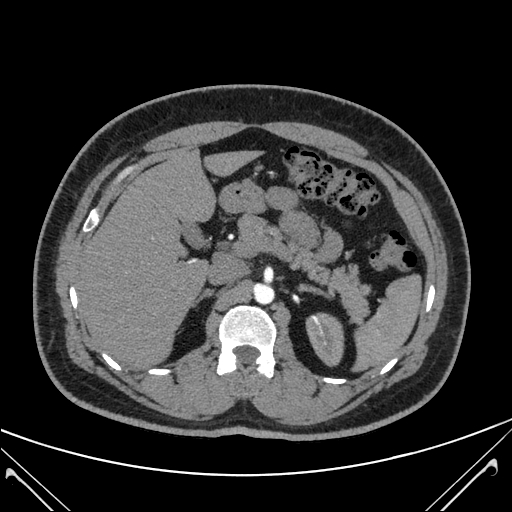
\includegraphics[width=2.7cm, height=1.4cm]{Normal- (1).jpg}};
\node[font=\footnotesize\bfseries, text=greenbr!70!black] at (12.35,-0.12) {Normal};
\node[inner sep=0pt, draw=redbr, line width=0.5pt]
  at (12.35,-1.05)
  {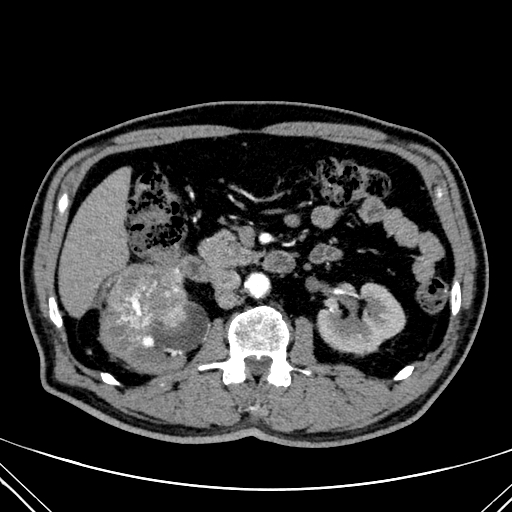
\includegraphics[width=2.7cm, height=1.4cm]{Tumor- (319).jpg}};
\node[font=\footnotesize\bfseries, text=redbr!70!black] at (12.35,-1.90) {Tumor};

%-- V: Métricas
\node[font=\footnotesize\bfseries] at (15.95, 1.90) {Métricas};
\draw[black!20, line width=0.5pt] (14.50,1.63) -- (17.40,1.63);
\foreach \y/\lbl in {1.10/Acurácia, 0.50/Precisão, -0.10/Recall,
                     -0.70/F1-Score, -1.35/{Mat.~Confusão}}
  \node[font=\footnotesize] at (15.95,\y) {\lbl};

\end{tikzpicture}
\caption{Diagrama geral da metodologia proposta.}
\label{fig:pipeline}
\end{figure*}

\subsection{Conjunto de Dados}

O conjunto de dados utilizado é o \textit{CT Kidney Dataset:
Normal-Cyst-Tumor and Stone}~\cite{dataset}, disponível na plataforma Kaggle.
O dataset contém 12.446 imagens únicas de tomografia computadorizada
distribuídas em quatro classes: cistos (3.709), rins normais (5.077), pedras
(1.377) e tumor (2.283). Para este trabalho, foram utilizadas apenas as
classes \textit{Normal} e \textit{Tumor}.

\subsection{Arquiteturas de CNNs}

Foram avaliadas cinco arquiteturas de CNNs pré-treinadas na base ImageNet,
todas consolidadas na literatura de visão computacional. Em todos os modelos
adotou-se a estratégia de aprendizado por transferência: as camadas
convolucionais, responsáveis pela extração de características, foram mantidas
congeladas com os pesos pré-treinados, e apenas a camada de classificação
final foi substituída por uma nova camada totalmente conectada com duas
saídas, correspondentes às classes Normal e Tumor, sendo a única treinada
para a tarefa em questão.

As redes da família \textit{ResNet} (\textit{Residual Neural Network}) foram
introduzidas por He et al.~\cite{he2016} em 2016 e caracterizam-se pelo
empilhamento de blocos residuais com conexões de atalho, que somam a entrada
de um bloco diretamente à sua saída. Esse mecanismo viabiliza o treinamento
de redes muito profundas sem a degradação provocada pelo desaparecimento do
gradiente. Neste trabalho foram avaliadas três profundidades: a ResNet-18 e a
ResNet-34, com 18 e 34 camadas organizadas em blocos residuais simples, e a
ResNet-50, com 50 camadas estruturadas em blocos do tipo gargalo, que ampliam
a capacidade de representação com menor custo computacional.

A \textit{AlexNet}~\cite{krizhevsky2012}, vencedora do desafio ImageNet de
2012 por ampla margem, é composta por cinco camadas convolucionais seguidas
de três camadas totalmente conectadas. Foi a primeira arquitetura a
demonstrar a viabilidade da extração automática de características em larga
escala, rompendo o paradigma dos descritores projetados manualmente, e
introduziu o uso da função de ativação ReLU e o treinamento acelerado por
unidades de processamento gráfico.

A \textit{VGG-16}~\cite{simonyan2014}, desenvolvida por Simonyan e Zisserman
na Universidade de Oxford, deve seu nome ao grupo \textit{Visual Geometry
Group}. Sua principal característica é a profundidade obtida pelo
empilhamento sucessivo de pequenos filtros convolucionais de tamanho
$3{\times}3$, totalizando 16 camadas com pesos — 13 convolucionais e
três totalmente conectadas. Originalmente projetada para classificar imagens em
até mil categorias, recebe imagens na resolução de $224{\times}224$ pixels.

\subsection{Critérios de Inclusão e Exclusão}

Foram incluídas as classes \textit{Normal} e \textit{Tumor},
excluindo-se \textit{Cisto} e \textit{Pedra} por não serem relevantes ao
objetivo de discriminação entre tecido renal saudável e tumoral. Para
garantir equilíbrio entre as classes, foram selecionadas aleatoriamente
2.283 imagens da classe Normal (correspondendo ao total disponível da classe
Tumor), totalizando 4.566 imagens. O conjunto balanceado foi dividido de
forma estratificada nas proporções de 60\% treino (2.738 imagens), 20\%
validação (914 imagens) e 20\% teste (914 imagens), com semente aleatória
$s{=}42$ para reprodutibilidade. A Fig.~\ref{fig:pipeline} ilustra o fluxo
completo desde a seleção dos dados até a avaliação.

\subsection{Pré-processamento}

Foram avaliadas três condições de pré-processamento, mantendo um grupo base
sem realce de contraste para fins de comparação.

\textbf{Base (sem realce).} As imagens são convertidas para escala de cinza
em 8 bits e replicadas nos três canais RGB para compatibilidade com os pesos
pré-treinados no ImageNet.

\textbf{CLAHE} (\textit{Contrast Limited Adaptive Histogram Equalization}).
Técnica que divide a imagem em $M_x{\times}M_y$ \textit{tiles} locais e
equaliza o histograma de cada \textit{tile} com limitação do contraste máximo.
Seja $I : \Omega \to \{0,\ldots,L{-}1\}$ uma imagem com $N$ pixels e
$L = 256$ níveis, o histograma normalizado é:

\begin{equation}
    p(r) = \frac{h(r)}{N}, \quad r \in \{0,\ldots,L-1\}.
    \label{eq:pmf}
\end{equation}

\noindent A equalização global obtém a CDF $F(r) = \sum_{s=0}^{r} p(s)$ e
aplica $T(r) = \lfloor (L{-}1)\cdot F(r) \rfloor$. Na CLAHE, o histograma
local de cada \textit{tile} $\mathcal{T}_{ij}$ é recortado no limite
$C = \beta\,N_t / L$, em que $N_t = w\,h$ é o número de pixels do \textit{tile}
e $\beta$ o fator de recorte de contraste:

\begin{equation}
    h_c(r) = \min\!\bigl(h_{ij}(r),\; C\bigr),
    \label{eq:clip}
\end{equation}

\noindent sendo o excesso redistribuído uniformemente antes da equalização
local, com interpolação bilinear nas bordas dos \textit{tiles}. Neste trabalho
adotou-se fator de recorte $\beta{=}2{,}0$ e divisão da imagem em uma grade de
$8{\times}8$ \textit{tiles}~\cite{clahe}.

\textbf{Correção Gama.} Aplica um mapeamento não-linear pixel a pixel:

\begin{equation}
    I_{\text{out}}(x,y) = \left(\frac{I_{\text{in}}(x,y)}{255}\right)^{\!\gamma}
    \!\times\; 255,
    \label{eq:gamma}
\end{equation}

\noindent com $\gamma{=}0{,}7$. Para $\gamma{<}1$, a curva clareia
seletivamente regiões escuras sem saturar as já contrastadas, evidenciando
padrões texturais de baixo contraste característicos de massas tumorais em
TC~\cite{gonzalez2018}.

Após a técnica selecionada, todas as imagens seguem o mesmo fluxo final:
conversão para RGB, redimensionamento para $224{\times}224$ px e normalização
canal a canal com os parâmetros ImageNet:

\begin{equation}
    \tilde{x}_c = \frac{x_c - \mu_c}{\sigma_c},\quad c\in\{R,G,B\},
    \label{eq:norm}
\end{equation}

\noindent com $\boldsymbol{\mu}{=}[0{,}485,\,0{,}456,\,0{,}406]$ e
$\boldsymbol{\sigma}{=}[0{,}229,\,0{,}224,\,0{,}225]$.

\subsection{Parâmetros de Treinamento e Avaliação}

O treinamento foi conduzido por 100 épocas, com otimizador Adam, taxa de
aprendizado de $1{,}0\times10^{-4}$, lote de 32 amostras e semente aleatória
$s{=}42$. Como função de perda adotou-se a entropia cruzada
(\textit{Cross-Entropy}) com duas saídas, sendo a predição final dada pela
classe de maior probabilidade. Os pesos correspondentes à época de maior
acurácia de validação foram retidos e empregados na avaliação sobre o
conjunto de teste.

\subsection{Avaliação dos Modelos}

Os modelos foram avaliados no conjunto de teste (914 amostras), com classe
positiva definida como Tumor ($TP$: verdadeiros positivos; $TN$: verdadeiros
negativos; $FP$: falsos positivos; $FN$: falsos negativos):

\begin{equation}
\text{Acurácia} = \frac{TP+TN}{TP+TN+FP+FN},
\label{eq:acc}
\end{equation}

\begin{equation}
\text{Precisão} = \frac{TP}{TP+FP},
\label{eq:prec}
\end{equation}

\begin{equation}
\text{Recall} = \frac{TP}{TP+FN},
\label{eq:recall}
\end{equation}

\begin{equation}
F_1 = 2\cdot\frac{\text{Precisão}\times\text{Recall}}{\text{Precisão}+\text{Recall}},
\label{eq:f1}
\end{equation}

\begin{equation}
\mathcal{L}(y,\hat{p}) = -\sum_{c\in\{0,1\}} y_c \log \hat{p}_c.
\label{eq:loss}
\end{equation}

\noindent Adicionalmente, foram analisadas matrizes de confusão e curvas de
acurácia e perda por época para as condições CLAHE e Gama.

\subsection{Recursos Computacionais}

Os experimentos foram executados em um servidor equipado com o NVIDIA GB10
Grace Blackwell Superchip, que integra processador ARM Cortex-X925
(10~núcleos) e Cortex-A725 (10~núcleos) com 128~GB de memória unificada
compartilhada entre CPU e GPU, eliminando transferências explícitas entre
os dois componentes. O ambiente de software utilizou Python~3.10.20,
PyTorch~2.12.0, TorchVision~0.27.0 (ambos com suporte a CUDA~13.0),
OpenCV, NumPy, Pandas, Scikit-Learn e Matplotlib.

% ─────────────────────────────────────────────────────────────────────────────
\section{Resultados e Discussão}

\subsection{Resultados no Conjunto de Teste}

A Tabela~\ref{tab:resultados} apresenta as métricas de teste dos 15
experimentos. Resultados em negrito indicam o melhor valor por modelo.

\begin{table}[htbp]
\caption{Métricas no Conjunto de Teste (914 amostras)}
\label{tab:resultados}
\begin{center}
\renewcommand{\arraystretch}{1.2}
\setlength{\tabcolsep}{3.5pt}
\begin{tabular}{llcccc}
\toprule
\textbf{Modelo} & \textbf{Cond.} &
\textbf{Acc.\,(\%)} & \textbf{Prec.\,(\%)} &
\textbf{Rec.\,(\%)} & \textbf{F1\,(\%)} \\
\midrule
\multirow{3}{*}{ResNet-18}
 & Base  & 96,94 & \textbf{97,35} & 96,50 & 96,92 \\
 & CLAHE & 95,19 & 95,38 & 94,97 & 95,18 \\
 & Gama & \textbf{97,48} & 97,17 & \textbf{97,81} & \textbf{97,49} \\
\midrule
\multirow{3}{*}{ResNet-34}
 & Base  & 95,19 & 95,58 & 94,75 & 95,16 \\
 & CLAHE & 95,40 & 95,21 & \textbf{95,62} & 95,41 \\
 & Gama & \textbf{96,06} & \textbf{97,30} & 94,75 & \textbf{96,01} \\
\midrule
\multirow{3}{*}{ResNet-50}
 & Base  & 95,73 & 95,43 & 96,06 & 95,75 \\
 & CLAHE & 96,06 & \textbf{96,67} & 95,40 & 96,04 \\
 & Gama & \textbf{96,50} & 96,50 & \textbf{96,50} & \textbf{96,50} \\
\midrule
\multirow{3}{*}{AlexNet}
 & Base  & 98,91 & \textbf{98,48} & 99,34 & 98,91 \\
 & CLAHE & 97,16 & 96,95 & 97,37 & 97,16 \\
 & Gama & \textbf{99,02} & 98,28 & \textbf{99,78} & \textbf{99,02} \\
\midrule
\multirow{3}{*}{VGG-16}
 & Base  & 98,91 & 98,06 & 99,78 & 98,92 \\
 & CLAHE & 98,36 & \textbf{99,11} & 97,59 & 98,35 \\
 & Gama & \textbf{99,12} & 98,28 & \textbf{100,00} & \textbf{99,13} \\
\bottomrule
\end{tabular}
\end{center}
\end{table}

\subsection{Impacto do Pré-processamento}

\textbf{Arquiteturas ResNet.} A correção gama ($\gamma{=}0{,}7$) beneficiou
consistentemente todas as arquiteturas ResNet, com ganhos de $+0{,}54$ p.p.\
(ResNet-18), $+0{,}87$ p.p.\ (ResNet-34) e $+0{,}77$ p.p.\ (ResNet-50) sobre a
condição base.
O mapeamento não linear da \eqref{eq:gamma} clareia regiões escuras
correspondentes a tecido tumoral de baixo contraste espontâneo, evidenciando
padrões que os blocos residuais exploram com maior eficiência. O CLAHE
produziu queda de $-1{,}75$ p.p.\ na ResNet-18 e ganhos discretos nas demais
($+0{,}21$ p.p.\ na ResNet-34 e $+0{,}33$ p.p.\ na ResNet-50), sugerindo que
os artefatos de borda entre \textit{tiles} perturbam sobretudo as ativações
das primeiras camadas convolucionais das redes mais rasas.

\textbf{AlexNet e VGG-16.} AlexNet e VGG-16 atingiram $98{,}91\%$ na condição
base, superando as ResNets (entre $95\%$ e $97\%$). O CLAHE causou queda de
$-1{,}75$ p.p.\ na AlexNet ($97{,}16\%$) e queda menor de $-0{,}55$ p.p.\ na
VGG-16 ($98{,}36\%$). A correção gama, por ser uma transformação monotônica
suave, elevou o desempenho de ambas: a AlexNet atingiu $99{,}02\%$ e a VGG-16
alcançou \textbf{99,12\%}, melhor resultado global do experimento, com
revocação de $100\%$ na classe Tumor. O comportamento é atribuído ao
classificador denso de três camadas totalmente conectadas presente em ambas
as redes: o CLAHE altera a distribuição de ativações de forma incompatível
com os padrões aprendidos na base ImageNet, enquanto a correção gama preserva
a ordem relativa das intensidades.


\begin{figure*}[!t]
\centerline{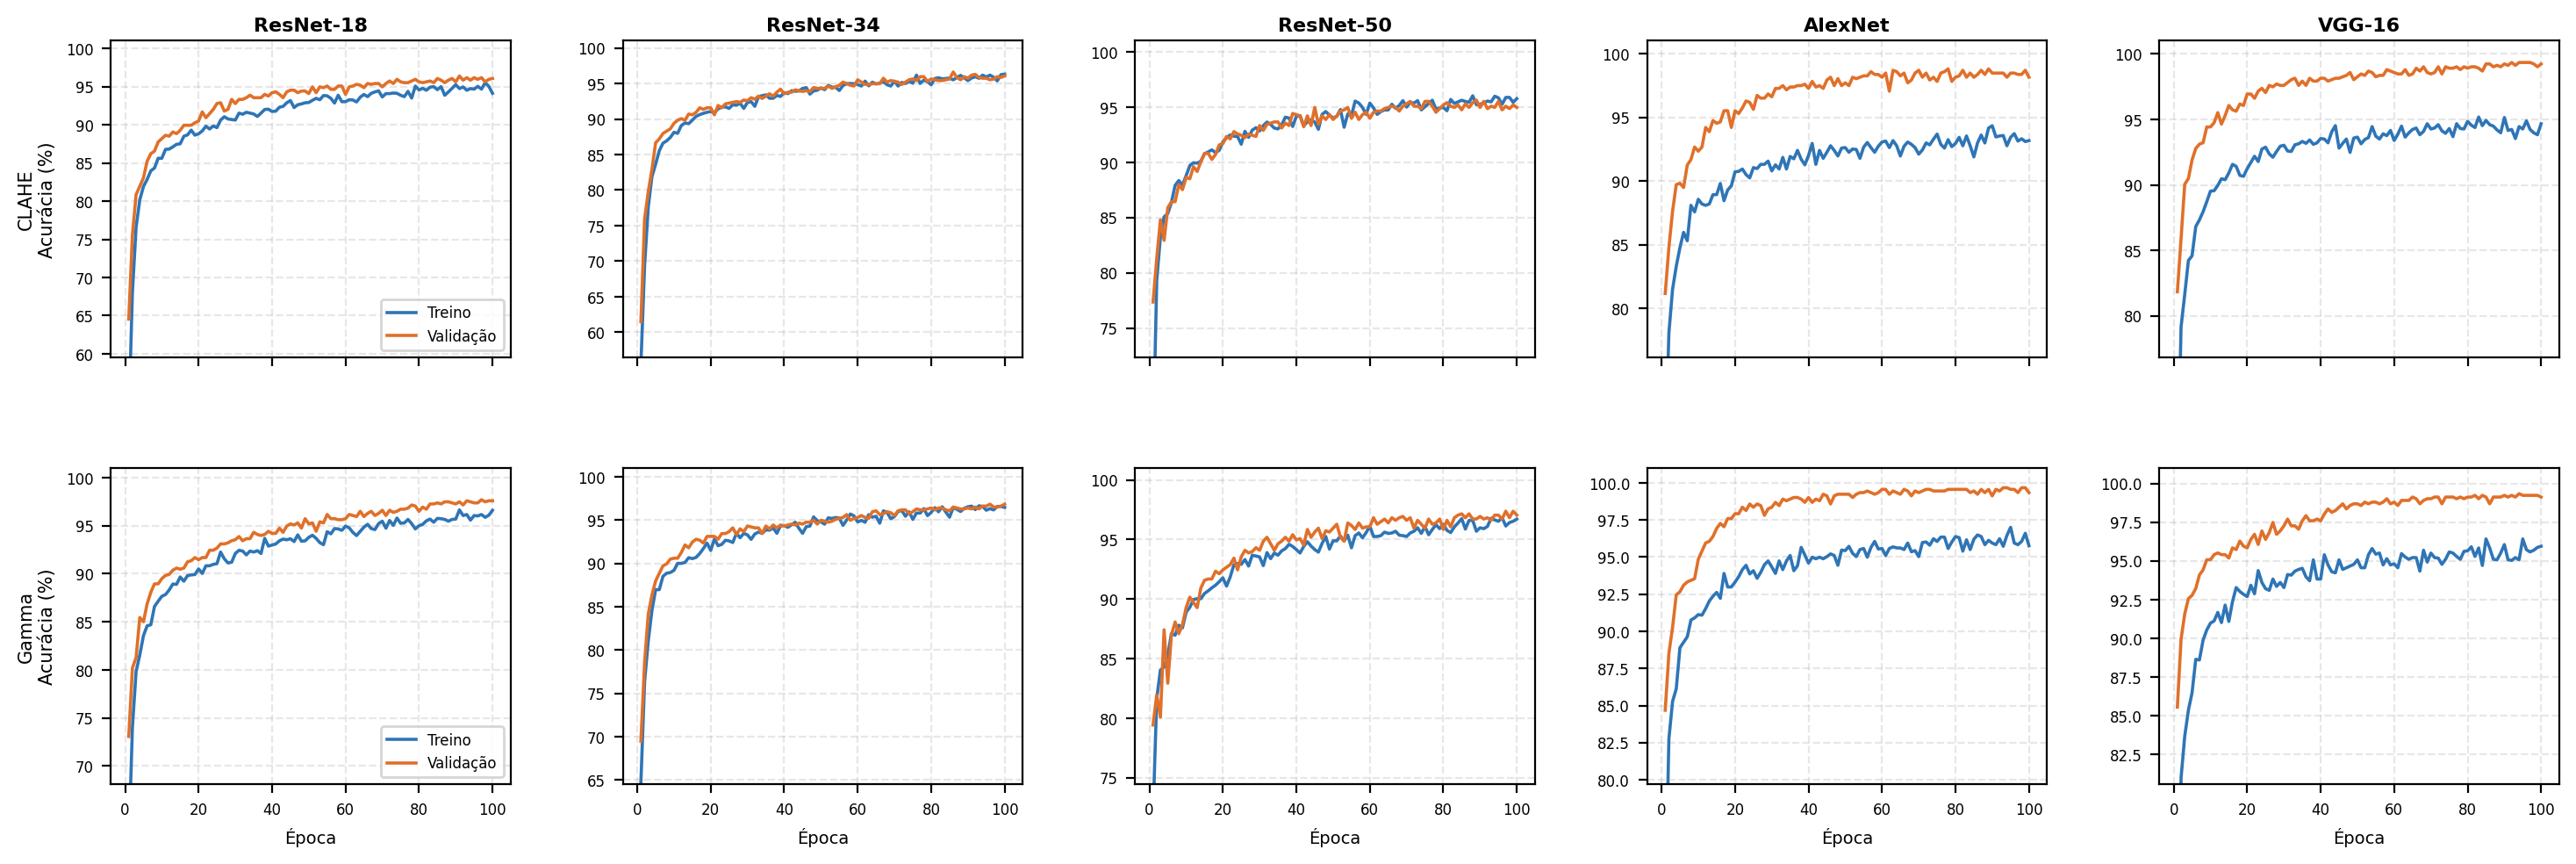
\includegraphics[width=\textwidth]{fig_acc_curves.png}}
\caption{Curvas de acurácia por época (100 épocas). Linha azul: treino.
Linha laranja: validação. Linha superior: condição CLAHE.
Linha inferior: condição Gama.}
\label{fig:acc_curves}
\end{figure*}

\begin{figure*}[!t]
\centerline{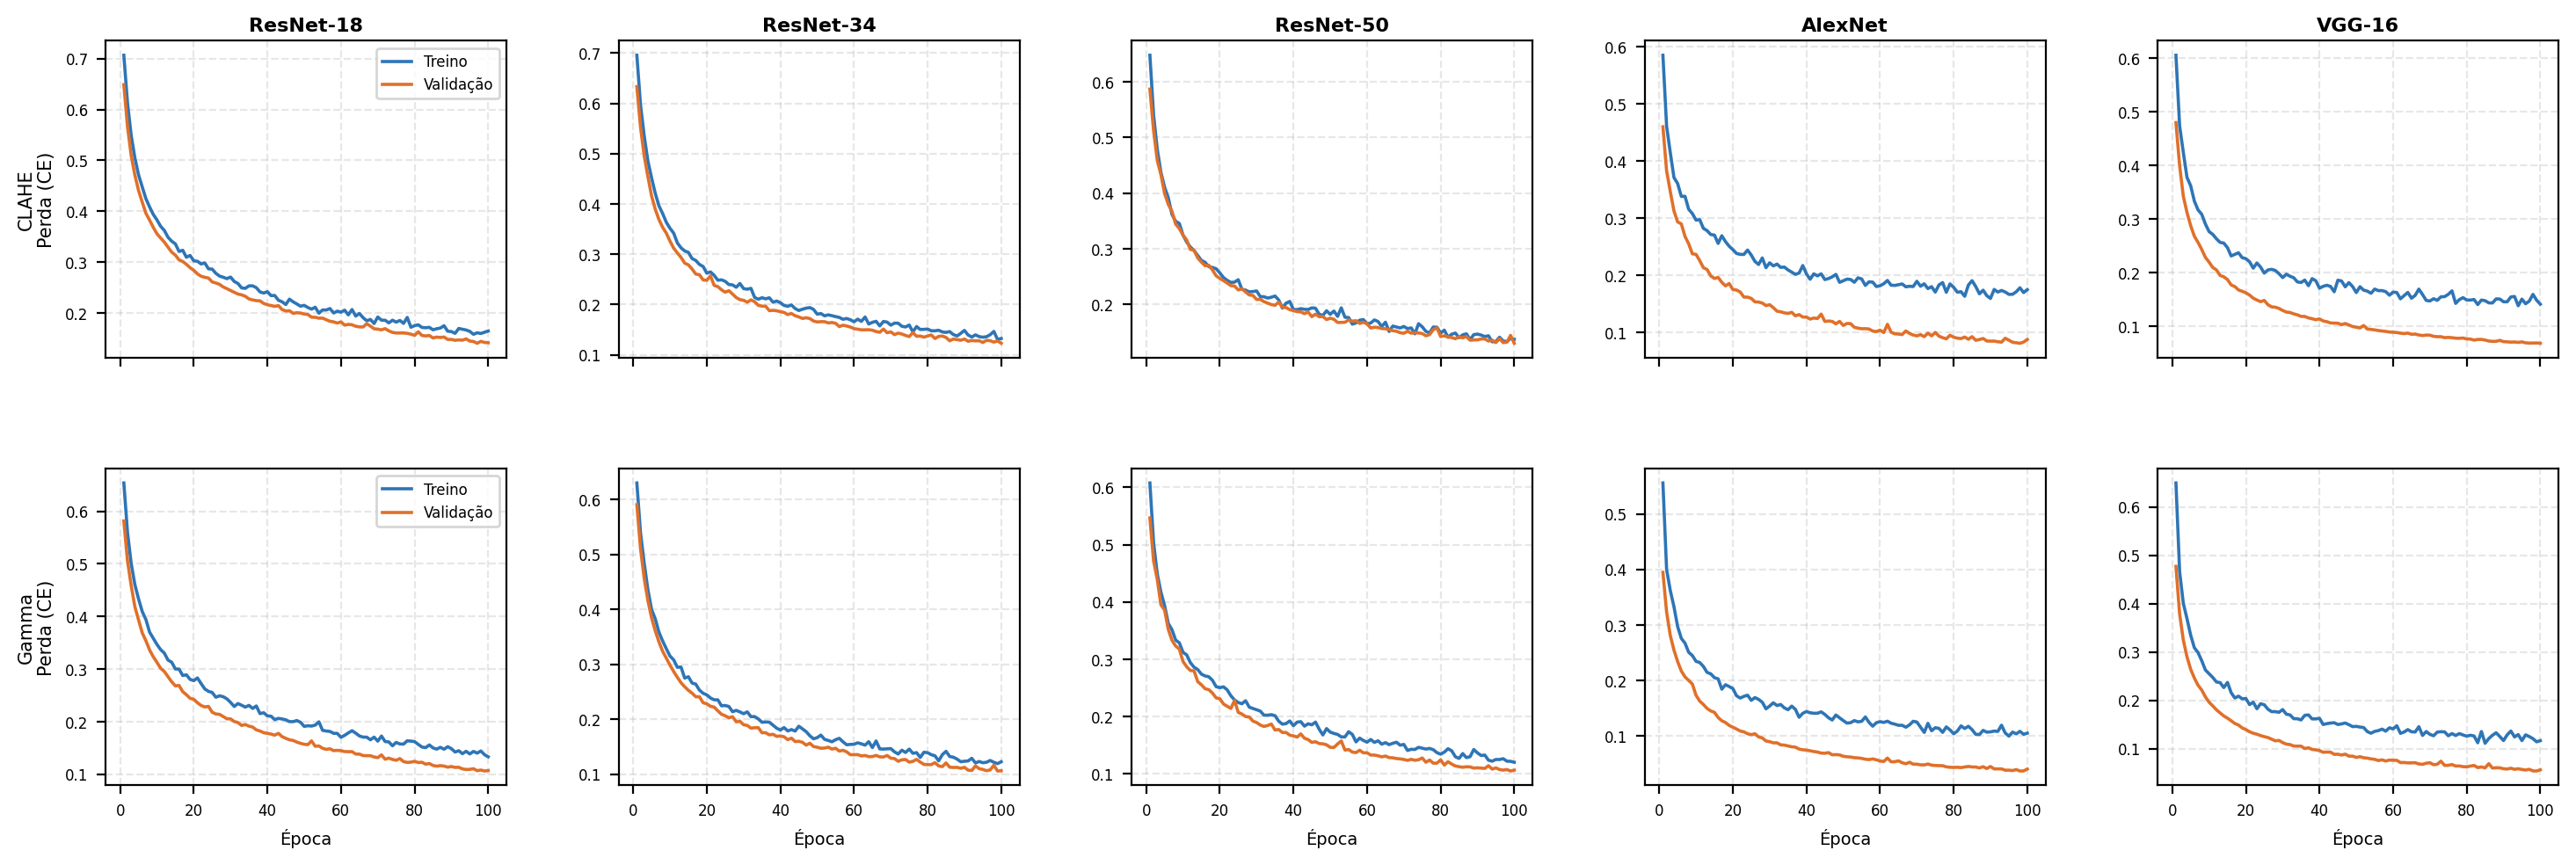
\includegraphics[width=\textwidth]{fig_loss_curves.png}}
\caption{Curvas de perda (\textit{Cross-Entropy}) por época.
Linha azul: treino. Linha laranja: validação.
Linha superior: CLAHE. Linha inferior: Gama.}
\label{fig:loss_curves}
\end{figure*}

\begin{figure*}[!t]
\centerline{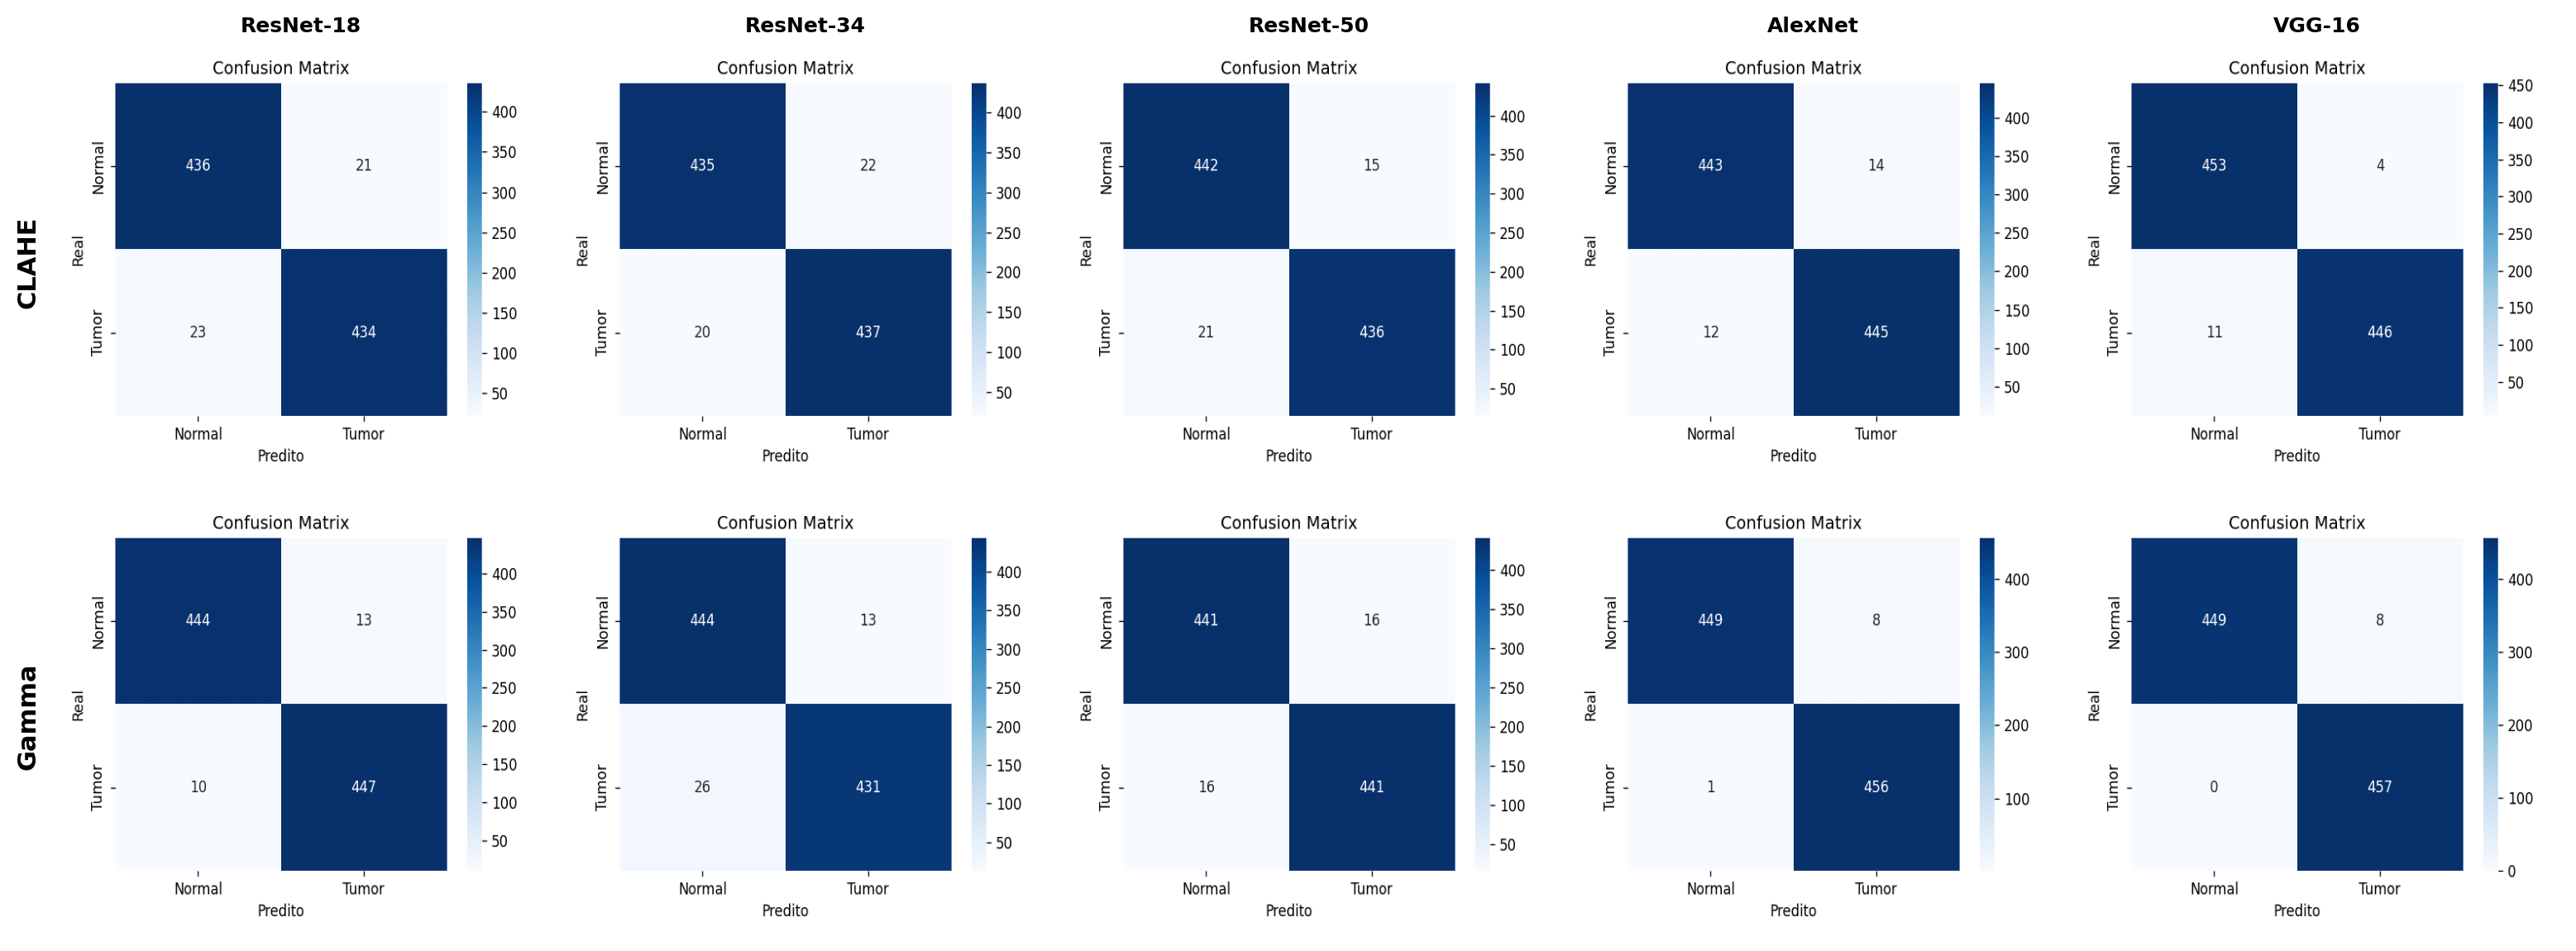
\includegraphics[width=\textwidth]{fig_confusion.png}}
\caption{Matrizes de confusão no conjunto de teste (914 amostras).
Linha superior: CLAHE. Linha inferior: Gama. Colunas: ResNet-18,
ResNet-34, ResNet-50, AlexNet, VGG-16.}
\label{fig:confusion}
\end{figure*}


\subsection{Curvas de Treinamento}

As Figs.~\ref{fig:acc_curves} e~\ref{fig:loss_curves} mostram as curvas de
acurácia e perda por época para as condições CLAHE e Gama. Para as ResNets,
o Gama antecipa a convergência e eleva o \textit{plateau} de validação,
enquanto o CLAHE apresenta maior variabilidade nas épocas intermediárias.
Para AlexNet e VGG-16, ambas as condições alcançam acurácias elevadas nas
primeiras épocas, evidenciando a eficácia do \textit{transfer learning} mesmo
com \textit{backbone} congelado. Em todas as arquiteturas, o reduzido intervalo
entre as curvas de treino e validação indica boa capacidade de generalização,
sem sinais expressivos de sobreajuste ao longo das 100 épocas avaliadas.

\subsection{Matrizes de Confusão}

A Fig.~\ref{fig:confusion} apresenta as matrizes de confusão no conjunto de
teste para todas as combinações modelo $\times$ condição (CLAHE e Gama).
Para as ResNets, o Gama reduz os falsos negativos (Tumor classificado como
Normal) em relação ao CLAHE, propriedade clinicamente relevante em
rastreamento oncológico, uma vez que erros nessa direção correspondem a
diagnósticos perdidos. AlexNet e VGG-16 apresentam erros próximos de zero
na condição base e resultados competitivos com o Gama; em particular, a
VGG-16 com correção gama atingiu revocação de $100\%$ na classe Tumor,
eliminando completamente os falsos negativos no conjunto de teste.

\FloatBarrier
% ─────────────────────────────────────────────────────────────────────────────
\section{Conclusão}

Este trabalho investigou sistematicamente o impacto das técnicas de
pré-processamento CLAHE e correção gama sobre o desempenho de cinco
arquiteturas CNN na classificação de câncer renal em imagens tomográficas.

A correção gama com $\gamma{=}0{,}7$ demonstrou ser a
técnica de pré-processamento mais consistente entre as avaliadas, sendo a
única que beneficiou todas as cinco arquiteturas sem exceção: os ganhos
variaram de $+0{,}11$ p.p.\ na AlexNet a $+0{,}87$ p.p.\ na ResNet-34.
O melhor resultado global foi obtido
pela VGG-16 com correção gama, que alcançou $99{,}12\%$ de acurácia e
revocação de $100\%$ na classe Tumor, evidenciando o potencial da técnica para
reduzir falsos negativos em cenários de rastreamento oncológico.

O CLAHE, por sua vez, apresentou comportamento variável: reduziu o desempenho
da ResNet-18 e da AlexNet em $-1{,}75$ p.p.\ cada, enquanto produziu ganhos
discretos nas ResNets mais profundas. Esse comportamento sugere que a
equalização adaptativa por \textit{tiles} pode introduzir artefatos de borda
incompatíveis com os filtros aprendidos na base ImageNet, com impacto mais
acentuado em redes com menor profundidade ou maior sensibilidade à distribuição
de intensidades.

Como trabalhos futuros, propõe-se avaliar diferentes valores de $\gamma$ por
arquitetura, estender a classificação para as classes Cisto e Pedra presentes
no dataset, e investigar estratégias de ajuste fino parcial das camadas
convolucionais.

\section*{Agradecimentos}

Os autores agradecem ao Laboratório LSI pela disponibilização dos recursos
computacionais utilizados na condução dos experimentos, sem os quais o
treinamento das arquiteturas avaliadas não seria viável no escopo deste trabalho.

% ─────────────────────────────────────────────────────────────────────────────
\begin{thebibliography}{00}

\bibitem{gomes2025}
C. A. Gomes, M. E. C. P. de Mello, R. S. F. Alves, G. B. Vaz,
R. W. Lerner, J. M. de Queiroz Salek, C. C. Norberto, e M. V. Copello,
``Qualidade de vida em pacientes oncológicos: impactos
do tratamento e estratégias de manejo,''
\textit{Brazilian Journal of Implantology and Health Sciences},
v.~7, n.~10, pp.~739--750, 2025.

\bibitem{santos2025}
V. M. P. Santos, A. C. Patrocinio, W. C. S. Carvalho, e P. M. de Sousa,
``Renal cancer classification in tomographic images using convolutional
neural networks to assist early diagnosis,''
\textit{Revista de Informática Teórica e Aplicada (RITA)},
v.~32, n.~1, pp.~61--66, 2025.

\bibitem{inca2022}
Instituto Nacional de Câncer (INCA),
``Estimativa 2023: incidência de câncer no Brasil,''
Rio de Janeiro: INCA, 2022.

\bibitem{campbell2021}
T. Powles, L. Albiges, A. Bex, E. Comperat, V. Grünwald, R. Kanesvaran,
H. Kitamura, R. McKay, C. Porta, G. Procopio, M. Schmidinger, C. Suarez,
J. Teoh, G. de Velasco, M. Young, e S. Gillessen,
``Renal cell carcinoma: ESMO clinical practice guidelines,''
\textit{Annals of Oncology}, v.~32, n.~11, pp.~1347--1359, 2021.

\bibitem{hall}
J. E. Hall e M. E. Hall,
\textit{Guyton \& Hall Tratado de Fisiologia Médica}, 14.~ed.
Rio de Janeiro: Elsevier, 2021.

\bibitem{bakas}
M. J. Sheller, G. A. Reina, B. Edwards, J. Martin, e S. Bakas,
``Multi-institutional deep learning modeling without sharing patient data,''
\textit{Nature Communications}, v.~11, n.~1, p.~5021, 2020.

\bibitem{vogel2019}
C. Vogel, B. Ziegelmüller, B. Ljungberg, K. Bensalah, A. Bex, S. Canfield,
R. H. Giles, M. Hora, M. A. Kuczyk, A. S. Merseburger, T. Powles, L. Albiges,
F. Stewart, A. Volpe, A. Graser, M. Schlemmer, C. Yuan, T. Lam, e M. Staehler,
``Imaging in suspected renal-cell carcinoma: systematic review,''
\textit{Clinical Genitourinary Cancer}, v.~17, n.~2, pp.~e345--e355, 2019.

\bibitem{klontzas2024}
M. E. Klontzas, G. Kalarakis, E. Koltsakis, T. Papathomas, A. H. Karantanas,
e A. Tzortzakakis,
``Convolutional neural networks for the differentiation between benign and
malignant renal tumors with a multicenter international computed tomography
dataset,''
\textit{Insights into Imaging}, v.~15, art.~26, 2024.

\bibitem{lecun2015}
Y. LeCun, Y. Bengio, e G. Hinton,
``Deep learning,''
\textit{Nature}, v.~521, pp.~436--444, 2015.

\bibitem{litjens2017}
G. Litjens, T. Kooi, B. E. Bejnordi, A. A. A. Setio, F. Ciompi,
M. Ghafoorian, J. A. W. M. van der Laak, B. van Ginneken, e C. I. Sánchez,
``A survey on deep learning in medical image analysis,''
\textit{Medical Image Analysis}, v.~42, pp.~60--88, 2017.

\bibitem{heller2021}
N. Heller, F. Isensee, K. H. Maier-Hein, X. Hou, C. Xie, F. Li, et al.,
``The state of the art in kidney and kidney tumor segmentation in
contrast-enhanced CT imaging: Results of the KiTS19 challenge,''
\textit{Medical Image Analysis}, v.~67, art.~101821, 2021.

\bibitem{uhm2021}
K.-H. Uhm, S.-W. Jung, M. H. Choi, H.-K. Shin, J.-I. Yoo, S. W. Oh,
J. Y. Kim, H. G. Kim, Y. J. Lee, S. Y. Youn, S.-H. Hong, e S.-J. Ko,
``Deep learning for end-to-end kidney cancer diagnosis on multi-phase
abdominal computed tomography,''
\textit{npj Precision Oncology}, v.~5, art.~54, 2021.

\bibitem{he2016}
K. He, X. Zhang, S. Ren, e J. Sun,
``Deep residual learning for image recognition,''
in \textit{Proc. CVPR}, 2016, pp.~770--778.

\bibitem{clahe}
S. M. Pizer, E. P. Amburn, J. D. Austin, R. Cromartie, A. Geselowitz,
T. Greer, B. ter Haar Romeny, J. B. Zimmerman, e K. Zuiderveld,
``Adaptive histogram equalization and its variations,''
\textit{Computer Vision, Graphics, and Image Processing},
v.~39, n.~3, pp.~355--368, 1987.

\bibitem{gonzalez2018}
R. C. Gonzalez e R. E. Woods,
\textit{Digital Image Processing}, 4.~ed. New York: Pearson, 2018.

\bibitem{rajkumar2023}
K. Rajkumar, R. T. S. Ramoju, T. Balelly, S. Ashadapu, Ch. R. Prasad, e Y. Srikanth,
``Kidney cancer detection using deep learning models,''
in \textit{Proc. ICOEI}, IEEE, 2023, pp.~1197--1203.

\bibitem{alzubi2022}
D. Alzu'bi, M. Abdullah, I. Hmeidi, R. AlAzab, M. Gharaibeh, M. El-Heis,
K. H. Almotairi, A. Forestiero, A. M. Hussein, e L. Abualigah,
``Kidney tumor detection and classification based on deep learning,''
\textit{Journal of Healthcare Engineering}, v.~2022, p.~3861161, 2022.

\bibitem{hadjiyski2020}
N. Hadjiyski,
``Kidney cancer staging: deep learning neural network based approach,''
in \textit{Proc. EHB}, IEEE, 2020, pp.~1--4.

\bibitem{dataset}
``CT Kidney Dataset: Normal-Cyst-Tumor and Stone,'' Kaggle, 2022.
Disponível em: kaggle.com/datasets/nazmul0087/\linebreak[1]
ct-kidney-dataset-normal-cyst-tumor-and-stone.

\bibitem{krizhevsky2012}
A. Krizhevsky, I. Sutskever, e G. E. Hinton,
``ImageNet classification with deep convolutional neural networks,''
in \textit{Proc. NeurIPS}, 2012, pp.~1097--1105.

\bibitem{simonyan2014}
K. Simonyan e A. Zisserman,
``Very deep convolutional networks for large-scale image recognition,''
in \textit{Proc. ICLR}, 2015.

\end{thebibliography}

\end{document}
